\graphicspath{{content/chapters/2_background/figures/}}
\chapter{Background}
\label{chp:background}

In this chapter, background information on established classical noise reduction methods is provided. It explores Spectral Subtraction, Wiener Filtering, and MMSE-LSA estimation, that do not require reference signals. The basis of machine learning models, autoencoders, is introduced. Additionally, the chapter introduces the key evaluation metrics used to assess speech enhancement performance. Finally, a brief section outlines the progression of the project and relevant foundational knowledge.

\section{Spectral Subtraction}
\label{sec:spectral_subtraction}

Spectral Subtraction is one of the most widely used techniques for single-channel speech enhancement. The core idea is to estimate the noise spectrum from a noisy speech signal and subtract it from the observed spectrum to obtain a cleaner signal \cite{loizou2013speech}. It assumes that noise remains relatively stationary over short time frames, while speech is a dynamic, non-stationary signal.

The analog speech signal \(x(t)\) must be digitized into \(x[n]\), a discrete time signal. This digitisation must satisfy the Nyquist criterion, sampling at a rate at least twice the maximum frequency for accurate representation. However, sampling introduces limitations, such as quantisation noise and aliasing. If the sampling rate is too low, high-frequency components may fold into lower frequencies, misrepresenting the signal content \cite{loizou2013speech}.

\begin{figure}[h]
    \centering
    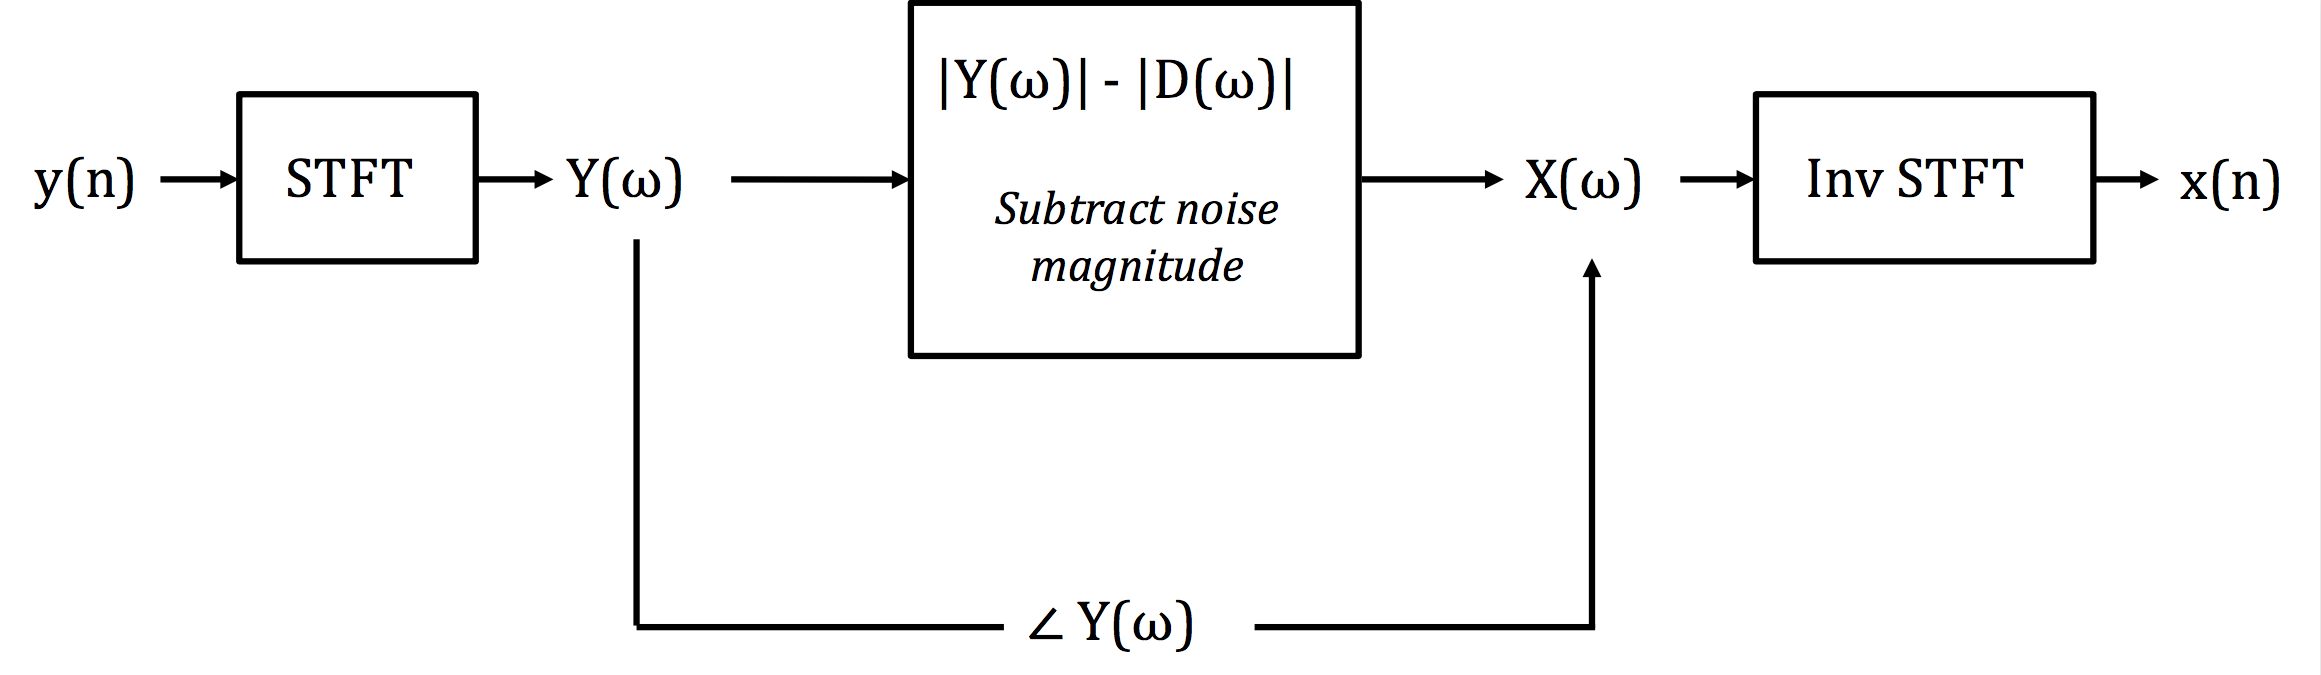
\includegraphics[width=\textwidth,keepaspectratio]{specsub.png}
    \caption{\label{fig:SSBlock} Block diagram of the Spectral Subtraction method \cite{dubey2016evaluation}.}
\end{figure}

Before applying spectral subtraction, the signal is pre-processed into a suitable format using the Short-Time Fourier Transform (STFT). The STFT segments the time-domain signal into overlapping frames using a windowing function and then converts each segment into the frequency domain. Windowing reduces spectral leakage and preserves continuity in the frequency domain. The magnitude spectrum of the noisy signal is obtained by taking the absolute value of the STFT \cite{dubey2016evaluation}. The noise spectrum is estimated by averaging the spectral magnitudes of non-speech segments over time. Once this estimate is obtained, it is subtracted from the noisy spectrum to yield an estimate of the clean speech. The final step applies the Inverse Short-Time Fourier Transform (ISTFT) to reconstruct the enhanced signal in the time domain by summing the overlapping frames.

This process can be mathematically described as:

\begin{equation}
    |X(\omega)| = |Y(\omega)| - |D(\omega)|
\end{equation}

where:
\begin{itemize}
    \item \( X(\omega) \): Estimated clean speech spectrum,
    \item \( Y(\omega) \): Magnitude spectrum of the noisy speech,
    \item \( D(\omega) \): Estimated noise spectrum.
\end{itemize}

Spectral subtraction is widely adopted due to its simplicity and low computational cost. It requires only a single input channel and is straightforward to implement. However, it assumes stationary noise, a condition often unmet in practice. It may alos introduce musical noise, a type of distortion perceived as tonal artifacts. Excessive subtraction may distort speech, while insufficient subtraction can leave residual noise.

Despite these challenges, spectral subtraction remains a valuable baseline for evaluating more advanced noise suppression techniques. Methods such as Wiener filtering and deep learning-based approaches have been developed to overcome these shortcomings through more adaptive or data-driven mechanisms \cite{loizou2013speech}.


\section{Wiener Filtering}
\label{sec:wiener_filtering}

Wiener filtering is a statistically grounded method for speech enhancement that aims to minimise the mean square error (MSE) between the estimated clean signal and the true clean signal \cite{loizou2013speech}. Originally developed for linear time-invariant systems, the Wiener filter assumes that both the signal and noise are stationary stochastic processes and seeks the optimal linear estimate of the clean speech given the noisy observation \cite{dubey2016evaluation}.

Though usable in time or frequency domains, the frequency version is preferred for efficiency and STFT compatibility. The key idea is that if the power spectral densities (PSDs) of the clean speech \(P_S(\omega)\) and the noise \(P_N(\omega)\) are known or can be estimated, the optimal filter \(H(\omega)\) is derived as:

\begin{equation}
    H(\omega) = \frac{P_S(\omega)}{P_S(\omega) + P_N(\omega)}
\end{equation}

This filter acts as a frequency dependent gain function. Frequencies where the clean speech dominates (\(P_S \gg P_N\)) are preserved, while noise dominant frequencies (\(P_N \gg P_S\)) are attenuated. The enhanced speech spectrum is obtained by multiplying the noisy spectrum \(Y(\omega)\) with the Wiener gain:

\begin{equation}
    \hat{X}(\omega) = H(\omega)Y(\omega)
\end{equation}

The enhanced signal is then reconstructed using the ISTFT.

\begin{figure}[h]
    \centering
    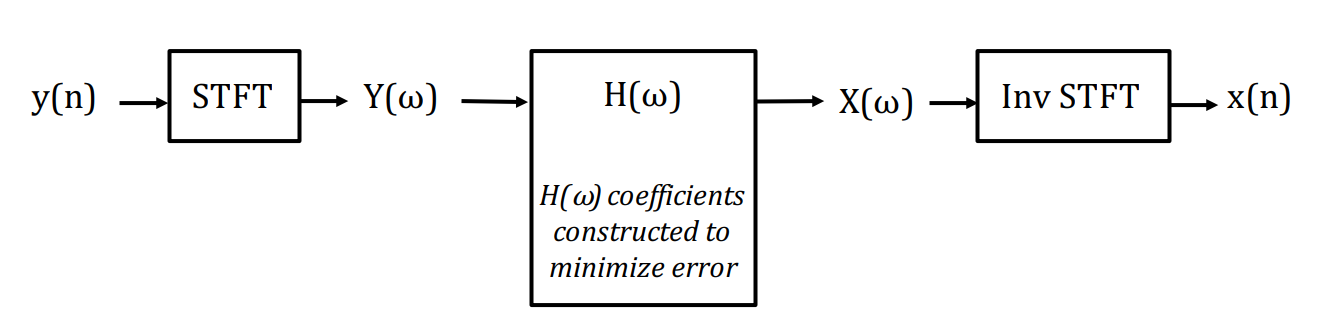
\includegraphics[width=0.95\textwidth,keepaspectratio]{wiener_block.png}
    \caption{\label{fig:WienerBlock} Block diagram of the Wiener filtering process \cite{dubey2016evaluation}.}
\end{figure}

Wiener filtering is a statistically optimal method that minimizes the mean square error (MMSE) between the estimated and clean speech signals. It performs well when noise characteristics can be reliably estimated, such as during silent speech segments, and is effective at preserving the spectral shape of speech components. However, the method assumes stationary, zero-mean noise uncorrelated with the speech signal. Assumptions that often fail in real-world, dynamic environments. This can lead to inaccurate power spectral density (PSD) estimates, resulting in performance degradation or over-smoothing that reduces intelligibility.

Despite these limitations, Wiener filtering remains a foundational approach in speech enhancement and is frequently integrated into more advanced or hybrid denoising pipelines \cite{dubey2016evaluation, loizou2013speech}.


\section{MMSE-LSA}
\label{sec:mmse_lsa}

The Minimum Mean-Square Error Log-Spectral Amplitude (MMSE-LSA) estimator is a statistically grounded single-channel speech enhancement technique first proposed by Ephraim and Malah in 1984~\cite{ephraim1984speech}. Unlike spectral subtraction and Wiener filtering, which operate on magnitude or power spectra. MMSE-LSA aims to minimise the mean-square error between the logarithm of the spectral amplitudes of the clean and enhanced speech signals.

The algorithm operates in the time/frequency domain, assuming additive noise and using the short-time Fourier transform (STFT) to decompose the noisy signal. It relies on estimates of the a priori and a posteriori signal-to-noise ratios (SNRs) to construct a gain function that enhances speech-dominant regions while suppressing noise. The enhanced spectral amplitude \( \hat{X}^{\text{LSA}}(\omega) \) is computed as:

\begin{equation}
    \hat{X}^{\text{LSA}}(\omega) = \exp \left( \mathrm{E} \left[ \log |X(\omega)| \,\big|\, Y(\omega) \right] \right)
\end{equation}

where \( Y(\omega) \) is the noisy observation and the expectation is taken over the distribution of the clean signal conditioned on the observed noisy spectrum.

A block diagram of the MMSE-LSA estimation process is shown in Figure~\ref{fig:mmse_lsa_block}. It begins with an STFT of the input signal, followed by separation into magnitude and phase. The magnitude spectrum is used to estimate the noise power spectral density (PSD), from which the a priori and a posteriori SNRs are derived. These estimates are then passed into the MMSE-LSA gain function, which produces a gain mask applied to the magnitude spectrum. The enhanced signal is reconstructed by combining the modified magnitude with the original phase, followed by the inverse STFT.

\begin{figure}[H]
    \centering
    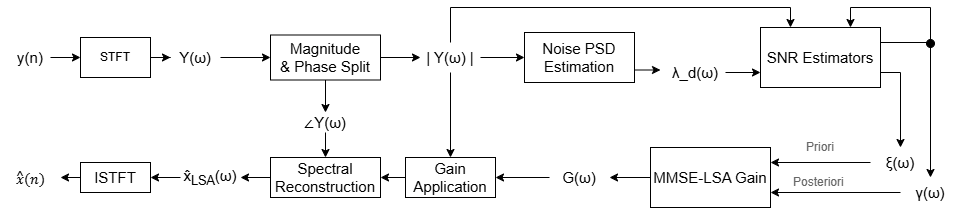
\includegraphics[width=\textwidth]{mmse-lsa.png}
    \caption{\label{fig:mmse_lsa_block} Block diagram of the MMSE-LSA method}
\end{figure}

The MMSE-LSA estimator incorporates a parametric model of the speech and noise distributions and uses recursive averaging to smooth SNR estimates across time frames. This results in a more adaptive and perceptually aligned gain function than traditional methods. This log-domain formulation better aligns with human auditory perception.

Despite its original formulation in the 1980s, MMSE-LSA continues to be a highly relevant technique. Numerous enhancements and application-specific variants have been developed in the 2010s and 2020s, including integrations with wavelet transforms~\cite{wei2016mmse}, improved noise tracking, and hybrid neural-DSP pipelines. This enduring relevance highlights MMSE-LSA's foundational robustness and its suitability for modern speech enhancement systems.

\section{Autoencoders}
\label{sec:autoencoders}

Machine learning (ML), a subset of artificial intelligence (AI), focuses on developing algorithms that enable systems to learn patterns from data and make decisions without being explicitly programmed. In the context of speech enhancement, ML techniques have enabled the development of specialised neural network architectures capable of recovering clean speech from noisy inputs. One widely used architecture is the \textit{autoencoder}, which learns to reconstruct its input through a compressed latent representation \cite{azarang2020review}.

\begin{figure}[h]
    \centering
    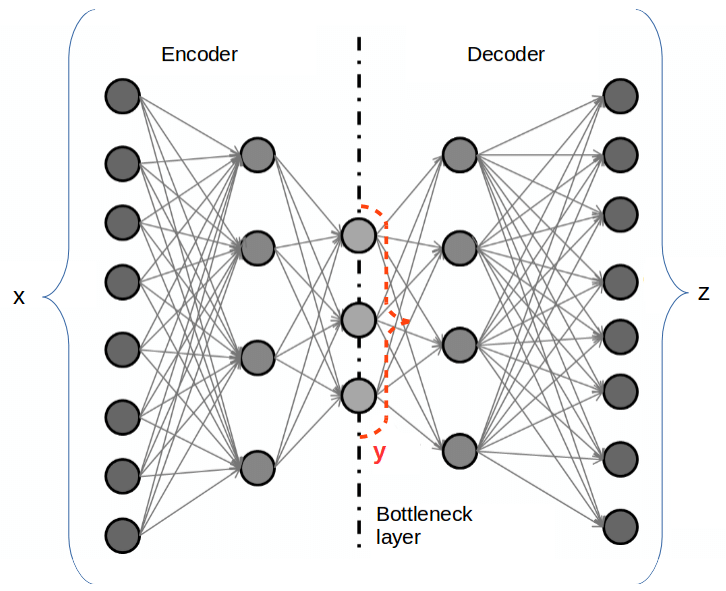
\includegraphics[width=0.5\textwidth,keepaspectratio]{autoencoder.png}
    \caption{\label{fig:autoencoder} Block diagram of an autoencoder architecture \cite{vachhani2017dae}.}
\end{figure}

An autoencoder consists of two main components: an encoder and a decoder. The encoder compresses the input signal \(x\) into a low-dimensional latent space using a series of convolutional, pooling, or fully connected layers. A central \textit{bottleneck} layer enforces this compression, encouraging the model to retain only the most salient features (speech structure) while discarding irrelevant noise.

The decoder reconstructs the signal \(y\) using upsampling or mirrored layers. The objective is to recover the clean speech signal with minimal reconstruction error. Autoencoders are trained using paired datasets of noisy and clean speech. During training, the noisy input is passed through the network, and the output is compared against the clean reference. The model is optimised to minimise the difference. Typically using a loss function such as Mean Squared Error (MSE) or Mean Absolute Error (MAE).

\begin{figure}[h]
    \centering
    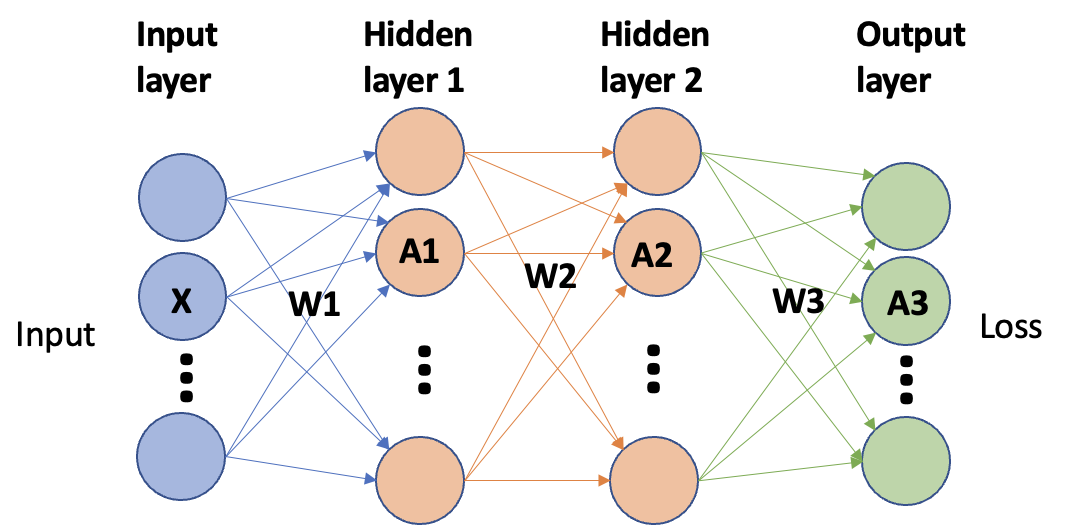
\includegraphics[width=0.5\textwidth,keepaspectratio]{weigths.png}
    \caption{\label{fig:weigths} Loss and weight update process in an autoencoder \cite{epoch2021}.}
\end{figure}

Training proceeds iteratively. A forward pass generates an output, and the loss function quantifies the error. This error is then propagated backward through the network via backpropagation to compute gradients, which are used to update the model’s weights using optimisers such as Stochastic Gradient Descent (SGD) or Adam. This process is repeated across many epochs until convergence.


\section{Evaluation Metrics}
\label{sec:evaluation_metrics}

To evaluate the performance of noise reduction algorithms, several objective metrics are commonly used. These metrics provide quantitative measures of the quality and intelligibility of enhanced speech signals when compared to their clean references. The following subsections describe the most widely adopted metrics in speech enhancement research, all of which are utilised in this project.

\subsection{Signal-to-Noise Ratio (SNR)}
\label{subsec:snr}

The Signal-to-Noise Ratio (SNR) is a fundamental metric that quantifies the relative strength of the desired speech signal compared to the background noise. A higher SNR indicates better separation between speech and noise components, which typically translates to improved intelligibility and perceived quality.

SNR is defined as:

\begin{equation}
    \text{SNR} = 10 \log_{10} \left( \frac{P_s}{P_n} \right)
\end{equation}

where \( P_s \) is the power of the clean speech signal and \( P_n \) is the power of the noise (or error) component. In practice, SNR can be computed in both time and frequency domains and is commonly used as a baseline performance indicator for denoising systems.

\subsection{Mean Squared Error (MSE)}
\label{subsec:mse}

The Mean Squared Error (MSE) measures the average squared difference between the enhanced and reference clean signals. It reflects the overall fidelity of the enhancement process but does not necessarily correlate with perceptual quality.

MSE is given by:

\begin{equation}
    \text{MSE} = \frac{1}{N} \sum_{n=1}^{N} (x(n) - \hat{x}(n))^2
\end{equation}

where \( N \) is the number of signal samples, \( x(n) \) is the clean signal, and \( \hat{x}(n) \) is the enhanced signal. Lower MSE values indicate better approximation of the clean signal.

\subsection{Perceptual Evaluation of Speech Quality (PESQ)}
\label{subsec:pesq}

The Perceptual Evaluation of Speech Quality (PESQ) is an objective metric designed to estimate the perceptual quality of speech, taking into account human auditory perception. Standardised \cite{itutp862}, PESQ is widely used in speech enhancement and telecommunication systems.

PESQ simulates the auditory perception process and compares the clean and enhanced signals using psychoacoustic models. The PESQ score ranges from -0.5 to 4.5, with higher scores indicating better perceptual quality. A score above 3.0 is generally considered acceptable for most applications.

\subsection{Short-Time Objective Intelligibility (STOI)}
\label{subsec:stoi}

The Short-Time Objective Intelligibility (STOI) metric is designed to assess the intelligibility of speech, especially in noisy or distorted conditions. It works by comparing the short-time spectral envelopes of clean and enhanced speech segments.

The STOI score lies between 0 and 1, where higher values indicate better intelligibility. Scores above 0.5 typically suggest acceptable levels of speech understanding. STOI is particularly useful when intelligibility, rather than perceptual quality alone, is of primary concern.

\subsection{Log Spectral Distance (LSD)}
\label{subsec:lsd}

The Log Spectral Distance (LSD) metric quantifies the spectral distortion introduced by a denoising algorithm. It measures the average distance between the logarithmic power spectra of the clean and enhanced signals across time and frequency.

LSD is defined as:

\begin{equation}
    \text{LSD} = \frac{1}{F} \sum_{f=1}^{F} \sqrt{ \frac{1}{T} \sum_{t=1}^{T} \left( \log S(f, t) - \log \hat{S}(f, t) \right)^2 }
\end{equation}

where \( S(f, t) \) and \( \hat{S}(f, t) \) are the clean and enhanced magnitude spectra at frequency bin \( f \) and time frame \( t \), respectively. Lower LSD values indicate better preservation of spectral characteristics and less distortion.

\vspace{2em}
Individually, these metrics suffer to provide complete meaningful evaluations of the performance of noise reduction algorithms. For example, SNR and MSE are sensitive to the absolute power levels of the signals, while PESQ and STOI focus on perceptual aspects. Thus, multiple metrics are needed for a well rounded assessment.


\section{Project Progression}
\label{sec:project_progression}

The initial objective of this project was to enhance speech signals corrupted by noise using traditional digital signal processing (DSP) techniques. The original scope involved implementing classical noise reduction methods, such as Spectral Subtraction and Wiener Filtering, with the intention of deploying them on an MSP432 microcontroller. These techniques were selected due to their low computational complexity and suitability for resource-constrained embedded systems.

However, early protyping in Python revealed inherent limitations of classical DSP methods. Particularly their poor performance in non-stationary noise and limited adaptability to diverse real-world conditions. While methods like Spectral Subtraction offer simplicity and efficiency, they often introduce musical noise artifacts and reduce intelligibility. Similarly, Wiener Filtering, though more rigorous, relies on assumptions about noise characteristics that may not hold in practice.

Meanwhile, data-driven approaches emerged as a compelling alternative. Real-time systems such as \textit{Krisp}, \textit{NVIDIA RTX Voice}, and \textit{RNNoise} demonstrate how machine learning-based models can robustly suppress noise by learning complex nonlinear mappings from large-scale clean/noisy speech datasets. Recognizing these advantages, the project evolved from solely implementing classical methods to exploring the deployment of lightweight machine learning-based speech enhancement models on more capable embedded processors. This shift aligned the project with modern trends while maintaining a focus on real-time deployment. It also enabled analysis of trade-offs between classical and data-driven methods in terms of performance, memory, and computation.

The revised project goal became benchmark machine learning-based noise suppression against classical DSP methods using objective metrics. The project title was thus updated from \textit{DSP Based Noise Cancellation System} to \textit{Machine Learning Noise Cancellation System} to reflect this shift in focus.